%; whizzy chapter
% -initex iniptex -latex platex -format platex -bibtex jbibtex -fmt fmt
% 以上 whizzytex を使用する場合の設定。

%     Kansai Debian Meeting resources
%     Copyright (C) 2007 Takaya Yamashita
%     Thank you for Tokyo Debian Meeting resources

%     This program is free software; you can redistribute it and/or modify
%     it under the terms of the GNU General Public License as published by
%     the Free Software Foundation; either version 2 of the License, or
%     (at your option) any later version.

%     This program is distributed in the hope that it will be useful,
%     but WITHOUT ANY WARRANTY; without even the implied warranty of
%     MERCHANTABILITY or FITNESS FOR A PARTICULAR PURPOSE.  See the
%     GNU General Public License for more details.

%     You should have received a copy of the GNU General Public License
%     along with this program; if not, write to the Free Software
%     Foundation, Inc., 51 Franklin St, Fifth Floor, Boston, MA  02110-1301 USA

%  preview (shell-command (concat "evince " (replace-regexp-in-string "tex$" "pdf"(buffer-file-name)) "&"))
% 画像ファイルを処理するためにはebbを利用してboundingboxを作成。
%(shell-command "cd image200708; ebb *.png")

%%ここからヘッダ開始。

\documentclass[mingoth,a4paper]{jsarticle}
\usepackage{kansaimonthlyreport}
\usepackage[dvips]{xy}

% 日付を定義する、毎月変わります。
\newcommand{\debmtgyear}{2009}
\newcommand{\debmtgdate}{25}
\newcommand{\debmtgmonth}{10}
\newcommand{\debmtgnumber}{28}

\begin{document}

\begin{titlepage}

% 毎月変更する部分、本文の末尾も修正することをわすれずに

 第\debmtgnumber{}回 関西 Debian 勉強会資料

\vspace{2cm}

\begin{center}
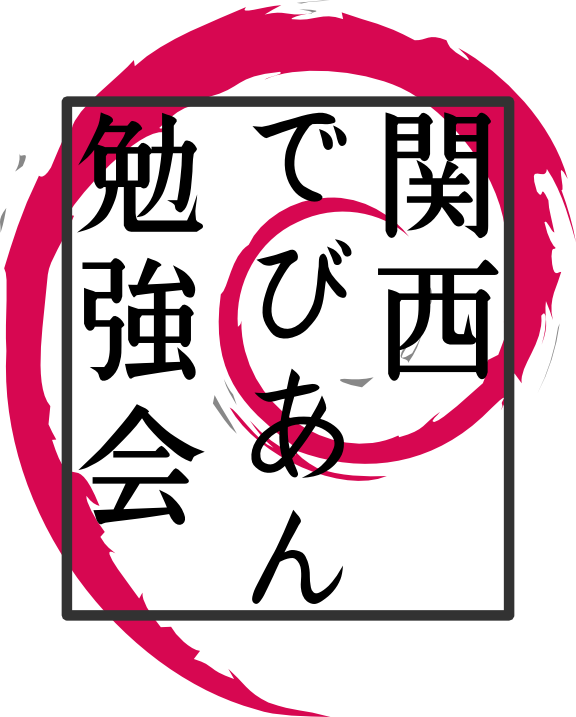
\includegraphics{image200802/kansaidebianlogo.png}
\end{center}

\begin{flushright}
\hfill{}関西 Debian 勉強会担当者 佐々木・倉敷・のがた\\
\hfill{}\debmtgyear{}年\debmtgmonth{}月\debmtgdate{}日
\end{flushright}

\thispagestyle{empty}
\end{titlepage}

\dancersection{Introduction}{Debian JP}

 関西 Debian 勉強会はDebian GNU/Linux のさまざ
 まなトピック(新しいパッケージ、Debian 特有の機能の仕組、Debian 界隈で起
 こった出来事、などなど)について話し合う会です。

 目的として次の三つを考えています。
 \begin{itemize}
  \item MLや掲示板ではなく、直接顔を合わせる事での情報交換の促進
  \item 定期的に集まれる場所
  \item 資料の作成
 \end{itemize}

 それでは、楽しいひとときをお過ごし下さい。

\newpage

\begin{minipage}[b]{0.2\hsize}
 {\rotatebox{90}{\fontsize{80}{80}
{\gt 関西デビアン勉強会}}}
\end{minipage}
\begin{minipage}[b]{0.8\hsize}
\hrule
\vspace{2mm}
\hrule
\setcounter{tocdepth}{1}
\tableofcontents
\vspace{2mm}
\hrule
\end{minipage}

%-------------------------------
\dancersection{最近の Debian 関係のイベント報告}{Debian JP}

\subsection{前回の関西 Debian 勉強会}

前回の関西Debian勉強会は、9月27日に京都リサーチパークにて開催されました。

関西Debian勉強会初の京都での開催でしたが、初参加の方も多く参加され、自己
紹介ではライトニングトークをされる方も続出して、かなり盛り上がりました。

発表は、のがたじゅんさんによる reportbugを使ってDebianのバグ報告をおこな
う方法の解説「GUIがついてかっこよくなったreportbugを使ってみよう」と、佐々
木洋平さんによるdebian.mentors.orgを利用して、Debianパッケージを公式リポ
ジトリに取り込んでもらうための流れを解説した「debian mentorsってご存知で
すか?」でした。

Debianのバグ報告の方法や、自作パッケージを公式リポジトリに取り込んでもら
うための流れがよくわかり、とてもよかったのではないでしょうか。

\begin{figure}[h]
 \begin{center}
 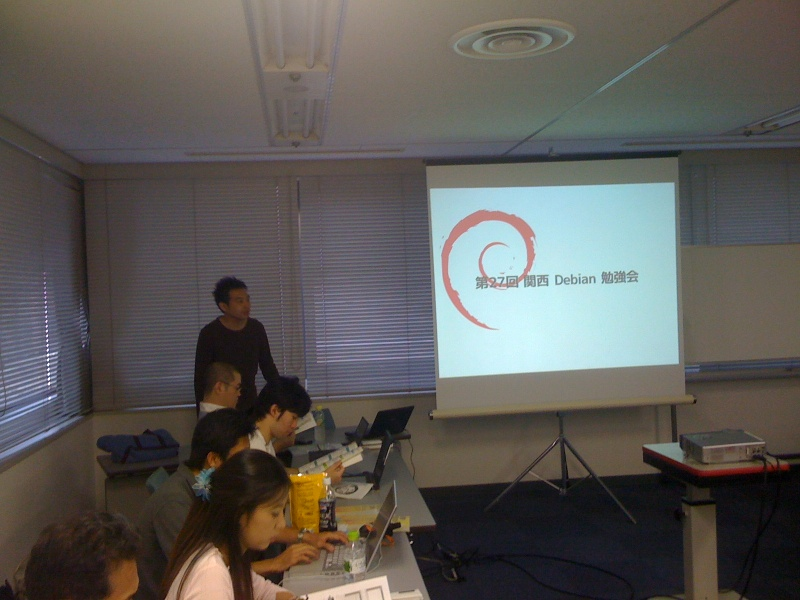
\includegraphics[width=6cm]{image200910/kyoto01.jpg}
 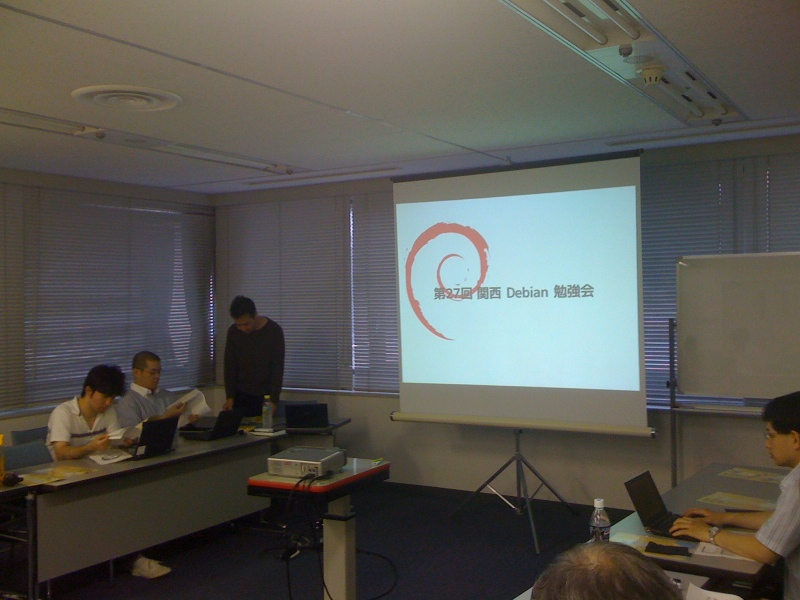
\includegraphics[width=6cm]{image200910/kyoto02.jpg}
 \caption{京都での勉強会の様子}
 \end{center}
\end{figure}


%-------------------------------
\dancersection{デバッグのお供:"gdbのススメ"}{杉本典充}

\makeatletter
   \renewcommand{\thetable}{%
   \thesection.\arabic{table}}
   \@addtoreset{table}{section}
\makeatother

\makeatletter
    \renewcommand{\thefigure}{%
    \thesection.\arabic{figure}}
    \@addtoreset{figure}{section}
\makeatother


\subsection{はじめに}
インターネットでは様々なオープンソースのプログラムが公開されています。それらのプログラムは開発者の手によるデバッグだけでなく、多くの人もデバッグ作業に参画することによって品質を高めていきます。そのデバッグ作業を終えたプログラムがいわゆる「安定したプログラム」であり、多くの人が安心して使えるレベルになるにはデバッグ作業はとても大切な作業の1つです。
今回は、Debianを使ってプログラムをデバッグする手法についてまとめてみました。

\subsection{gdbとは}
gdbとはGNU Debugger\footnote{GNU Debugger Webサイト
\url{http://www.gnu.org/software/gdb/}}のことで、C言語・C++向けのソースレベルデバッガです。開発者はgdbを使うことでプログラムが今どこの部分を実行しているか、プログラムの状態はどうなっているかを知ることができるため、デバッグ作業を効率的に行うことができます。
「man gdb(1)」によると、gdbには大きく4つの機能があると書かれています。
\begin{itemize}
 \item プログラムの動作を詳細に指定してプログラムを実行させる。
 \item 指定した条件でプログラムを停止させる。
 \item プログラムが止まった時に、何が起こったか調べる。
 \item バグによる副作用を修正し、別のバグを調べるためプログラムの状態を変更する。
\end{itemize}

gdbが使用する設定ファイルは"〜/.gdbinit"であり、gdbの初期設定値をこのファイルに定義することで変更できます。

\subsection{開発環境とgdbのインストール}
C言語のプログラムを開発するためにはコンパイラが必要です。gdbの他にプログラムを作成するために必要なソフトウェア一式もインストールします。
\begin{commandline}
$ sudo apt-get update
$ sudo apt-get install gcc make
$ sudo apt-get install gdb
\end{commandline}

環境も整ったところで、プログラムを作成します。今回は「FizzBuzz」\footnote{FizzBuzzとは、『1から100からまでの整数を標準出力に出力せよ。ただし、3で割り切れるときは「Fizz」、5で割り切れるときは「Buzz」、3と5の両方で割り切れるときは「FizzBuzz」と標準出力に出力せよ。』というプログラムの問題である。}といわれているプログラムを例にしてみます。

\subsection{gdbを使ってみましょう}
\subsubsection{まずはデバッグビルドします}
プログラムをgdbで操作するためにはプログラムにデバッグ情報を付与してビルドする必要があります。
gccのコンパイルオプション及びビルドオプションにデバッグシンボルを付与する"-g"オプションをつけてビルドします。(デバッグ時の最適化レベルは開発者によって指定が違うこともあります。ここでは最適化レベルは無指定(="-O0"、最適化なし)としてビルドします。)


\subsubsection{gdb単体でプログラムを追いかけてみる}
それではシェルからgdbを起動します。gdbを起動すると以下のような入力受付状態になります。

\begin{commandline}
$ gdb
GNU gdb 6.8-debian
Copyright (C) 2008 Free Software Foundation, Inc.
License GPLv3+: GNU GPL version 3 or later <http://gnu.org/licenses/gpl.html>
This is free software: you are free to change and redistribute it.
There is NO WARRANTY, to the extent permitted by law.  Type "show copying"
and "show warranty" for details.
This GDB was configured as "x86_64-linux-gnu".
(gdb) 
\end{commandline}

gdbのプロンプトでコマンドを入力することによりデバッガを通してプログラムを動かすことができます。
デバッグ作業でよく使うgdbのコマンドを表\ref{table_use_gdb}に示します。

\begin{table}[h]
\begin{center}
\caption{gdbを操作するコマンド(一部抜粋)}\label{table_use_gdb}
\begin{tabular}{|l|c|p{9cm}|}
\hline
コマンド & 省略コマンド & 説明 \\ \hline \hline
run (引数)& r & プログラムを最初から実行します。\\
 & & 引数を指定する場合は、runの後に引数を指定します。 \\ \hline
break (停止位置) & b & ブレークポイントを設定します。ブレークポイントは「関数名」と「ソースコード:行番号」のいずれかで指定できます。\\ \hline
delete (breakpoint番号)& d & ブレークポイントを削除します。単にdeleteだけを実行するとすべてのブレークポイントを削除します。\\ \hline
list & l & 現在実行中の近くのソースコードをある行数表示します。(初期設定値は10行)\\ \hline
step & s & ステップイン実行します。\\ \hline
next & n & ステップオーバー実行します。\\ \hline
finish & fin & ステップアウト実行します。\\ \hline
continue & c & 現在停止中の位置からプログラムを再開します。\\ \hline
print (変数名) & p & プログラム中の(変数名)の内容を表示します。ポインタ変数の場合は「print *ポインタ変数名」と指定することでポイントが指し示す値を表示できます。\\ \hline
set var (変数名)=(設定値) & なし & プログラム中の(変数名)の値を(設定値)に変更します。\\ \hline
quit & q & gdbを終了します。\\ \hline
attach (プロセスID)& なし & 実行中の(プロセスID)をgdbで制御できるようにします。\\ \hline
detach & なし & attach中のプロセスをgdbの制御下から切り離します。切り離されたプログラムはそのまま動作し続けます。\\ \hline
shell & なし & shellを起動します。shellをexitするとgdbプロンプトに戻ります。\\ \hline
help & h & gdbのコマンドに関するヘルプを表示します。\\ \hline
info (コマンド) & i & 様々な情報を表示します。\\ \hline
\end{tabular}
\end{center}
\end{table}

\subsection{gdbのフロントエンドツール}
gdbは単体でも十分デバッグ可能ですが、よりデバッグ作業を行いやすいようにgdbのフロントエンドツールが多くあります。
X Window System上で動作する統合開発環境(IDE)ではKDevelop、Anjuta、Eclipse、NetBeansなど、コマンドライン上でも動作するEmacs、Vimなどもフロントエンドとして利用することができます。

\subsubsection{Emacs GUDモードでgdbを使ってみる}
EmacsにはGUD(Grand Unified Debugger)という機能があり、Emacs上で様々なデバッガと連携することができる仕組みです。GUDはgdbに限らず、perldb(perl用デバッガ)やpdb(python用デバッガ)なども起動することができます。

Emacsの実行中に以下のキーを入力してgdbを起動します。

\begin{commandline}
M-x gdb
\end{commandline}

その後、ミニバッファで実行ファイルを指定してEnterキーを入力します。

\begin{commandline}
Run gdb (like this): gdb --annotate=3 ../a.out
\end{commandline}

すると図\ref{figure-emacs-gud1}、図\ref{figure-emacs-debugging1}のような画面に切り替わります。

\begin{figure}[H]
\begin{center}
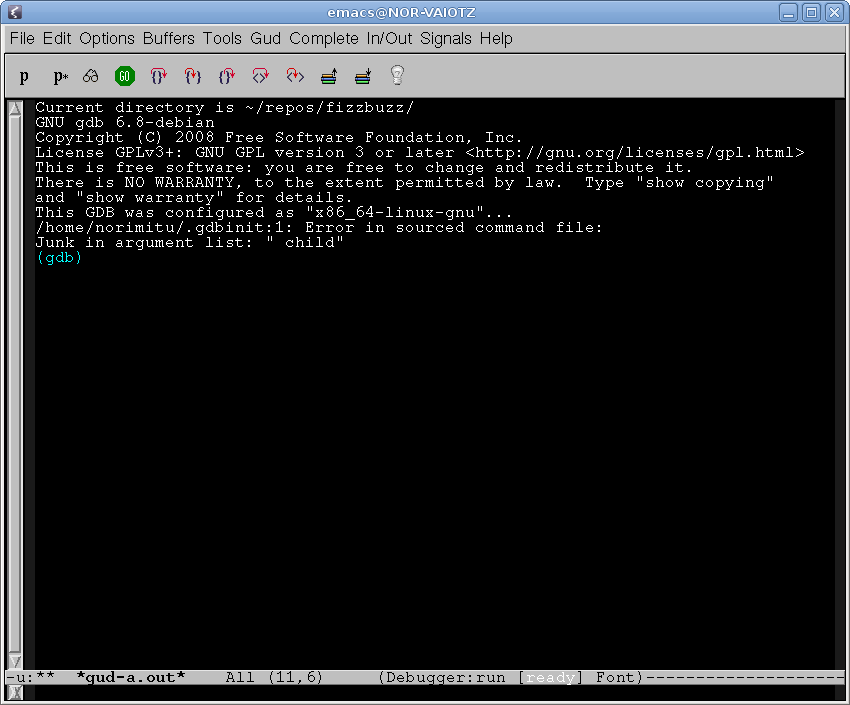
\includegraphics[scale=0.5]{image200910/gdb-emacs-gud1.png}
\caption{Emacs GUDモードでgdbを起動した画面(1)}\label{figure-emacs-gud1}
\end{center}
\end{figure}

\begin{figure}[H]
\begin{center}
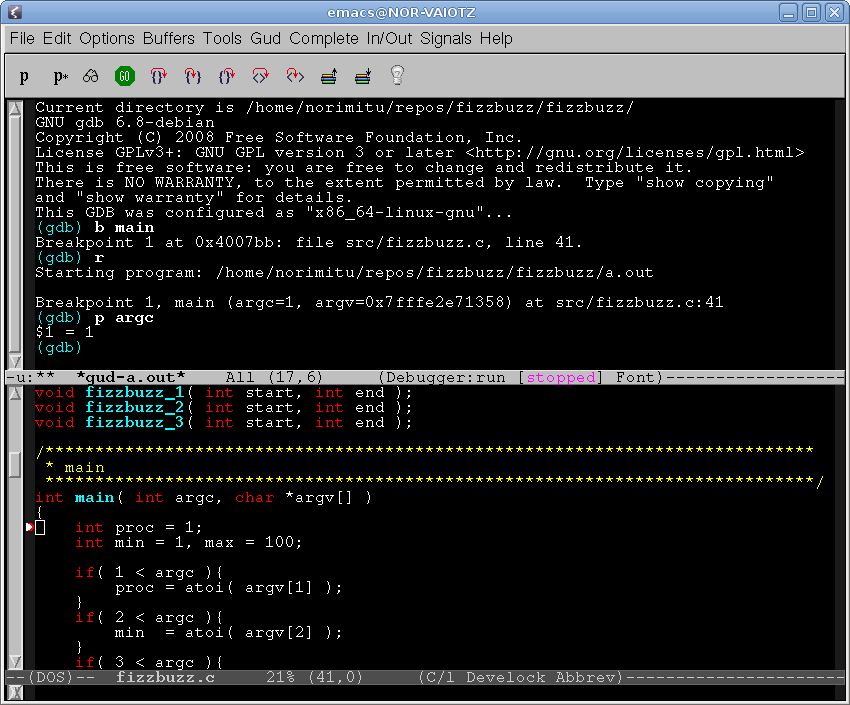
\includegraphics[scale=0.5]{image200910/gdb-emacs-gud2.png}
\caption{Emacs GUDモードでデバッグ中の画面(2)}\label{figure-emacs-debugging1}
\end{center}
\end{figure}


また、Emacsの設定ファイル"〜/.emacs.el"に「(setq gdb-many-windows t)」を指定しておくと、すると図\ref{figure-emacs-gud2}、図\ref{figure-emacs-debugging2}のような画面でgdbが起動します。
この画面を表示するには「gud.el」というファイルが必要であり。lennyの場合はEmacsをインストールすると一緒にインストールされます。

\begin{figure}[H]
\begin{center}
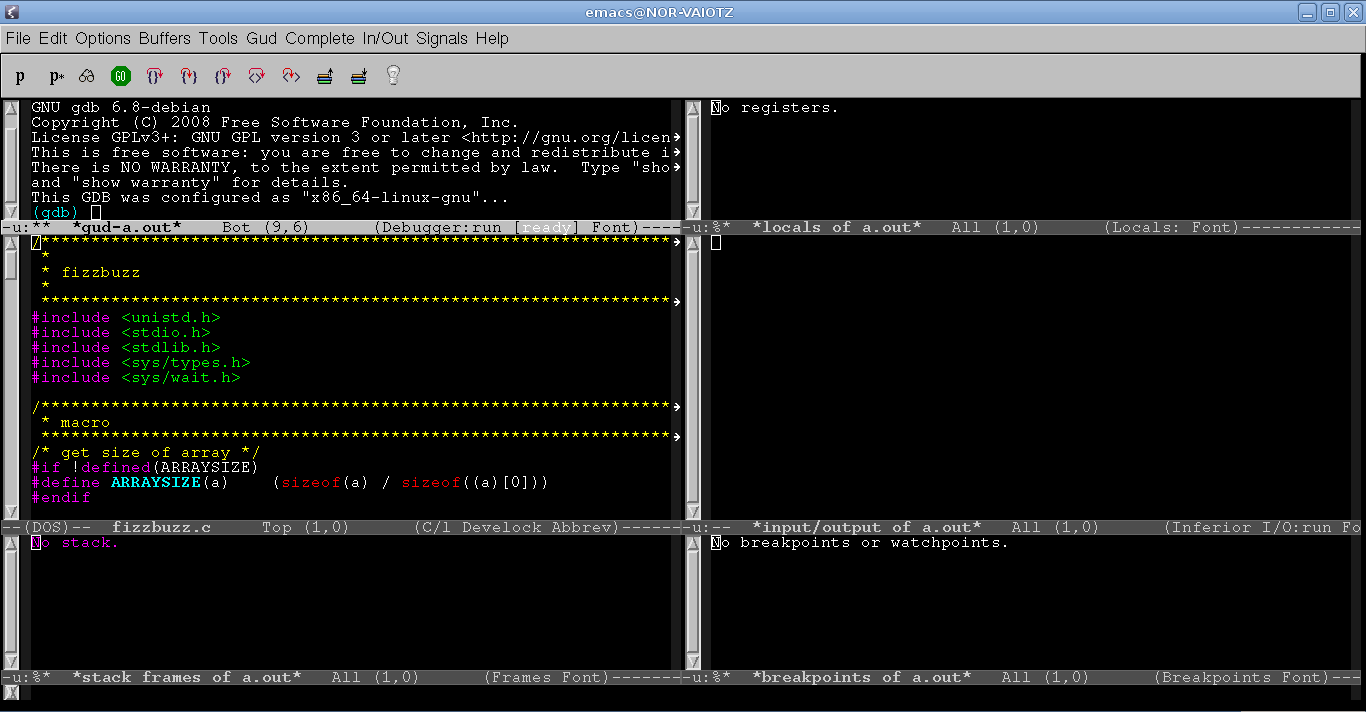
\includegraphics[scale=0.5]{image200910/gdb-emacs-gud3.png}
\caption{Emacs GUDモードでgdbを起動した画面(3)}\label{figure-emacs-gud2}
\end{center}
\end{figure}

\begin{figure}[H]
\begin{center}
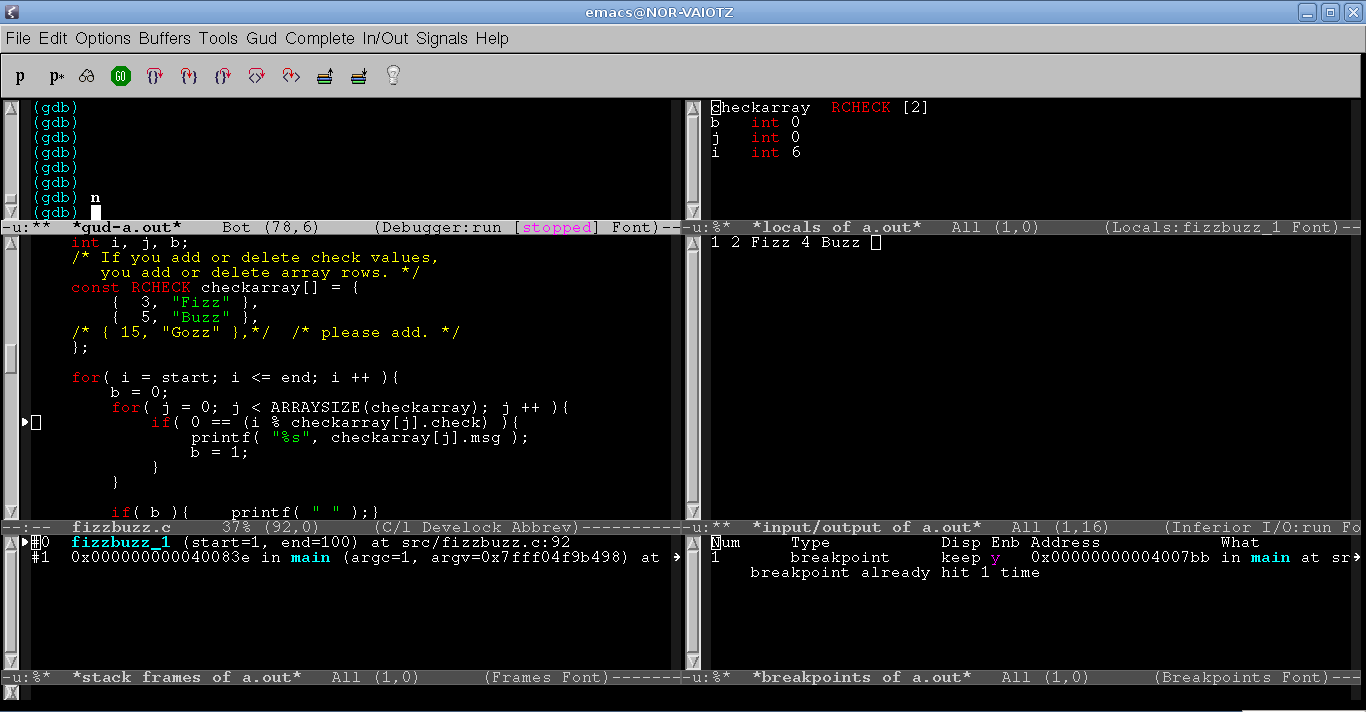
\includegraphics[scale=0.5]{image200910/gdb-emacs-gud4.png}
\caption{Emacs GUDモードでデバッグ中の画面(4)}\label{figure-emacs-debugging2}
\end{center}
\end{figure}


\subsection{いろいろなプログラムのデバッグ方法}
私がプログラムをgdbを使ってデバッグするときの操作例を挙げてみます。

\subsubsection{単発実行系プログラムのデバッグ}
単発実行するプログラムの場合はデバッガでプログラムの起動を行い、その後にデバッグ作業を開始することになります。

\begin{enumerate}
\item gdbを起動します。
\item breakコマンドでブレークポイントを指定します。(実際には「b main」と入力してプログラムの最初で止めることも多いです。)
\item runコマンドでプログラムを開始します。
\item stepコマンド、nextコマンドでプログラムを追いかけます。
\item デバッグが完了したら、continueコマンドで残りのプログラムすべてを実行します。
\item quitコマンドでgdbを終了します。
\end{enumerate}

\subsubsection{デーモン系プログラムのデバッグ}
デーモンとして動作しているプログラムの場合は、動作中のプログラムをgdbで制御する必要があるためアタッチする必要があります。

\begin{enumerate}
\item デバッグするデーモンプログラムを実行します。
\item デバッグするデーモンプロセスのプロセスIDを調べます。
\item gdbを起動します。
\item プロセスIDを指定してattachコマンドを実行し、デバッグするデーモンプロセスにアタッチします。
\item breakコマンドでブレークポイントを指定します。(おそらく無限ループ処理のどこかで停止させることになると思います。)
\item ブレークポイントを設定したところでプログラムが一時停止しますので、stepコマンドやnextコマンドを実行してプログラムを追いかけます。
\item デバッグが終了したら、detachコマンドでプロセスからデタッチします。
\item quitコマンドでgdbを終了します。
\end{enumerate}

\subsubsection{forkするプログラムのデバッグ}
forkするプログラムの場合、fork()後に親プロセスと子プロセスのどちらを追いかけるのかを「set follow-fork-mode parent」などと設定しておく必要があります。

\begin{enumerate}
\item gdbを起動します。
\item 「set follow-fork-mode」を設定し、fork()後にデバッガを追うプロセスを親プロセスにするか、子プロセスにするか設定します。
\item breakコマンドでブレークポイントを指定します。
\item runコマンドでプログラムを開始します。
\item fork()した後は「set follow-fork-mode」で指定した親プロセスか子プロセスのいずれかを追従しますのでそのまま続けてデバッグします。
\item quitコマンドでプログラムを終了します。
\end{enumerate}

\subsection{まとめ}
今回はgdbの紹介とEmacs GUDモードにおいてプログラムをデバッグする一例を紹介しました。Emacs GUDモードを使ったデバッグ操作はX Window System上だけでなくコンソール環境でも同様の手順で実行できるため、telnet環境やssh環境でも同じスタイルでプログラムのデバッグ作業を行うことができます。

みなさんもDebianを使ってたくさんデバッグしてみましょう。

\subsection{参考資料}
\begin{itemize}
 \item man gdb(1)
\end{itemize}

%-------------------------------
\dancersection{佐々木流 Debian パッケージの作り方。最初から最後まで}{佐々木洋平}

\subsection{はじめに}

...なんて{\bf 大それた}タイトルなんでしょう..%
私事で忙しくて訂正できなかった訳ですが、 我ながら恥ずしいです。

さて、 佐々木のパッケージ作成遍歴は以下の通りです:
\begin{enumerate}
      \item 売り物ソフトウェアを dpkg で管理するために弄り始める
      \item 自分達の作っているソフトウェアの deb パッケージを作成し始める。
      \item どうせなら本家に... $\leftarrow$ イマココ
\end{enumerate}
今日のお話は、 これらを踏まえての「パッケージ作成最初から最後まで」です。
ここでは「最初」を「ソースの取得」、「最後」を「lintian \& piuparts clean」
とします。 
個々の How to、 特に一番ハマりやすい {\tt debian/rules}については
時間の紙面の都合上参考文献へのポインタを示すに留めます。 是非質問して下さい。

\subsection{Package}

コンパイル後のソフトウェアなどをすぐ利用できる形に
まとめたものをバイナリパッケージと呼びます。 
%
Debian では拡張子が {\tt .deb} のファイルがこれにあたります。
%
我々は普段 {\tt apt-get}や{\tt aptitude} を利用して、 バイナリパッケージ
を導入/更新/削除したりしています。
%
バイナリパッケージは制御情報とデータを {\tt tar.gz}に圧縮し、 
バージョン情報とともに {\tt ar(1)} でまとめたものです。
%
これらは非常に一般的なコマンドですから、
バイナリパッケージを展開するだけならば多くのシステムで可能です。

バイナリパッケージに対して、 
これを作成するための素材をまとめたものをソースパッケージと言います。 
%
これは二つないし三つのファイルからなります:
\begin{itemize}
      \item オリジナルのソース一式({\tt .orig.tar.gz})
      \item パッケージの情報({\tt .dsc}))
      \item バイナリパッケージを作成するための変更({\tt .diff.gz})
    \begin{itemize}
          \item オリジナルのソースが無い場合
        (Debian 固有のパッケージ等)の場合は存在しない。
    \end{itemize}
\end{itemize}
ソースパッケージは
導入したり削除したりする性質のパッケージではありません。  
%
目的はバイナリパッケージの作成にあります。 
%
Debian が提供しているバイナリパッケージには、 
対応するソースパッケージが必ず存在しており、 
必要に応じてソースパッケージを取得してバイナリパッケージを構築する
ことができます。

\subsubsection{deb package inside}

{\tt dpkg-deb} コマンドを利用して、 実際にパッケージを展開してみましょう。
%
例えば rabbit\footnote{%
RD や Wiki フォーマットで記述したテキストをベースにした
プレゼンテーションツール。 この間 unstable に入りました!!} 
%
というパッケージの deb ファイルを展開してみると...
\begin{commandline}
  % dpkg-deb -x rabbit_0.6.1-1_all.deb rabbit
                 (rabbit というパッケージを rabbit というディレクトリに展開)
  % dpkg-deb -e rabbit_0.6.1-1_all.deb rabbit/DEBIAN        
                 (rabbit パッケージの制御情報を rabbit/DEBIAN に展開)
  % cd rabbit ls 
  DEBIAN/  usr/
  % tree 
  .
  |-- DEBIAN
  |   |-- control
  |   |-- md5sums
  |   `-- preinst
  `-- usr
      |-- bin
      |   |-- rabbit
-------- snip ---------------
      |   `-- rabbit-theme-manager
      |-- lib
      |   `-- ruby
      |       `-- 1.8
      |           |-- rabbit
-------- snip ---------------
      |         
      `-- share
          |-- doc
          |   `-- rabbit
          |       |-- NEWS.en.gz -> changelog.gz
-------- snip ---------------
          |       |-- README.Debian
          |       |-- README.en.gz
          |       |-- README.ja.gz
          |       |-- changelog.Debian.gz
          |       |-- changelog.gz
-------- snip ---------------
          ...
179 directories, 575 files
\end{commandline}
パッケージの制御情報は DEBIAN以下に展開しました。 
{\tt rabbit} の場合、 
\begin{commandline}
  % ls -R DEBIAN
  DEBIAN:
  control  md5sums  preinst*
\end{commandline}
の三つからなります。 これらは
\begin{description}
      \item[control] 
    メンテナの名前、 
    対応するソースパッケージ名、 依存関係などが記述されたファイル
      \item[md5sums]
    提供される各ファイルの md5 checksum
      \item[preinst]
    インストール作業の前に実行される hook シェルスクリプト。
    パッケージによっては、 
    {\tt preinst} 以外に
    {\tt postinst}、 {\tt prerm}、{\tt postrm} などが存在します。
\end{description}


パッケージのデータは {\tt usr} 以下に展開しました。
%
deb パッケージを導入した際には、 これらは {\tt /usr} 以下に展開されます。

というわけで上記構成になったディレクトリツリーを用意して
tar.gz で圧縮したりするとバイナリパッケージができあがります。

\subsubsection{余談: dpkg-deb でパッケージを再構築}
\label{subsubseclab:余談}

売り物の(ソースが取得できない)ソフトウェアを
Debian のパッケージシステムで管理したい
時に佐々木がよくやる手段は
\begin{itemize}
      \item {\tt alien} で rpm を deb に変換
      \item 上記 {\tt dpkg-deb -e|-x} でファイルを展開
      \item 適切に配置、 修正
      \item {\tt dpkg-deb -b} で再アーカイブ
\end{itemize}
として、 似非パッケージを作成することです。
当然配布はできませんが%
\footnote{売り物って rpm ばっかりです。Ubuntu のおかげで大分減りましたが。}
例として、 大昔の Intel Compiler Ver.8 のパッケージ作成は以下の様にやって
いました。
\begin{commandline}
 % tar xvzf l_cc_pc_8.1.028.tar.gz
 % cd l_cc_pc_8.1.028
 % rm -rf *64*
 % sudo alien *.rpm
 % rm *.rpm
 % sudo chown $USER *.deb
 % mkdir tmp
 % dpkg-deb -e intel-icc8_8.1-29_i386.deb tmp/DEBIAN
 % dpkg-deb -x intel-icc8_8.1-29_i386.deb tmp/
 % echo DESTINATION=/opt/`ls tmp/opt` >> tmp/DEBIAN/postinst
 % cat <<EOF >> tmp/DEBIAN/postinst
  for FILE in $(find $DESTINATION/bin/ -regex \
     '.*[ei](cc|fort|fc|cpc)$\|.*cfg$\|.*pcl$\|.*vars[^/]*.c?sh$' \
     2> /dev/null) do
      sed s@\@$DESTINATION@g $FILE > ${FILE}.abs
      mv ${FILE}.abs $FILE
      chmod 755 $FILE
  done
  for FILE in $(find $DESTINATION/bin/ -regex '.*[ei]cc' 2> /dev/null) do
      sed s@\@$DESTINATION@g $FILE > ${FILE}.abs
      mv ${FILE}.abs $FILE
      chmod 755 $FILE
  done
  for FILE in $(find $DESTINATION/bin/ -regex '.*[ei]cpc' 2> /dev/null) do
      sed s@\@$DESTINATION@g $FILE > ${FILE}.abs
      mv ${FILE}.abs $FILE
      chmod 755 $FILE
  done
  for FILE in $(find $DESTINATION/bin/ -regex '.*[ei]fort' 2> /dev/null) do
      sed s@\@$DESTINATION@g $FILE > ${FILE}.abs
      mv ${FILE}.abs $FILE
      chmod 755 $FILE
  done
  for FILE in $(find $DESTINATION/bin/ -regex '.*[ei]fc' 2> /dev/null) do
      sed s@\@$DESTINATION@g $FILE > ${FILE}.abs
      mv ${FILE}.abs $FILE
      chmod 755 $FILE
  done
 EOF
 % dpkg-deb -b tmp intel-icc8_8.1-29_i386.deb
 % dpkg -i intel-icc8_8.1-29_i386.deb
 % dpkg -i intel-iidb8_8.1-46_i386.deb
 % dpkg -i --force-overwrite intel-isubh8_8.1-29_i386.deb
\end{commandline}
最近は Intel Compiler に愛がない\footnote{%
マイナーバージョン上がる度にディレクトリ構成がコロコロ変わるので
つきあいきれなくなりました}
のでやっていませんが。

\subsection{パッケージ作成}

さて、 単にバイナリパッケージを作成するだけならば
前小節(\ref{subsubseclab:余談})で示した通り
\begin{itemize}
      \item DEBIAN 以下に control、 md5sums、 必要ならば hook スクリプト
      \item パッケージとして / 以下に展開したいディレクトリ構成に揃えた
    ファイル群
\end{itemize}
を作成して dpkg-deb でまとめれば良いだけです。 
%
ですが、 あんまり一般的ではありませんね。
%
以下では、 {\tt GNU hello} を例に\footnote{「またー?」とか言わないこと}、 
実際に配布まで含めたパッケージ作成方法について述べてみます。

\subsubsection{前準備} 

\paragraph{環境変数の設定}
パッケージメンテナの名前とメールアドレスを環境変数に設定します:
\begin{commandline}
DEBFULLNAME="Youhei SASAKI"; export DEBFULLNAME
DEBEMAIL=uwabami@gfd-dennou.org ; export DEBEMAIL
\end{commandline}
配布も考えているなら GPG 鍵の記述に合わせておくと良いと思います。

\paragraph{最低限必要なパッケージの導入}

{\tt build-essential} メタパッケージを導入しておきます。 このパッケージ
はdeb パッケージを構築するのに最低限必要となるパッケージを導入するメタ
パッケージです。 
%
具体的には
\begin{enumerate}
      \item {\tt libc6-dev}|{\tt libc-dev}
      \item {\tt g++}
      \item {\tt make}
      \item {\tt dpkg-dev}
\end{enumerate}
とこれに依存する幾つかのファイルが導入されます
\footnote{{\tt dpkg-dev} が {\tt make} に依存しているので、 
なんか変な気分ですが、 正しいんですよね? きっと…}。

\begin{commandline}
% apt-cache show build-essential
Package: build-essential
Priority: optional
Section: devel
Installed-Size: 48
Maintainer: Matthias Klose <doko@debian.org>
Architecture: amd64
Version: 11.4
Depends: libc6-dev | libc-dev, g++ (>= 4:4.3.1), make, dpkg-dev (>= 1.13.5)
Filename: pool/main/b/build-essential/build-essential_11.4_amd64.deb
Size: 7126
MD5sum: 86a942017ad93721c91212398a828a0c
SHA1: 5ac2ba90444e1eaed96b2163389a8812eb107b01
SHA256: 3dbd2e6b4e998412a6ad4d32b242523559b536168bcce7f227c7ce30256808a5
Description: Informational list of build-essential packages
 If you do not plan to build Debian packages, you don't need this
 package.  Starting with dpkg (>= 1.14.18) this package is required
 for building Debian packages.
 .
 This package contains an informational list of packages which are
 considered essential for building Debian packages.  This package also
 depends on the packages on that list, to make it easy to have the
 build-essential packages installed.
 .
----- snip -----
% sudo aptitude install build-essential
\end{commandline}

\paragraph{ソースの取得、 確認}
動かないソフトウェアをパッケージ化するのは大変ですよね?  事前にソースを
取得して動作確認しておくと良いでしょう。  また「動作させるために patch
を書いた!」という猛者は、 そのパッチを保管しておくと幸せになれるかもしれません。

{\tt GNU hello} は次の URL から取得できます。
\url{http://www.gnu.org/software/hello/}

{\tt GNU hello} は {\tt configure ; make ; make install} で導入する
ソフトウェアです。 実際に configure を動かしてみます。
\begin{commandline}
% cd hello-2.4
% ./configure 
...
\end{commandline}
エラーがでなければこれで終了です。
もし{\tt ./configure} が必要なファイルを探せずエラー終了する場合には、
{\tt apt-file} コマンドで必要なファイルを提供している
Debian パッケージを探してみましょう。
\begin{commandline}
% sudo aptitude install apt-file
% sudo apt-file update
% apt-file search [file 名]
\end{commandline}
足りないファイルを導入したら、 もう一度 {\tt ./configure} を走らせます。
これをくりかえして、 必要なファイルを導入していきます。

無事 {\tt ./configure} が通るようになったら {\bf make} を実行してみます。
\begin{commandline}
% make 
make all-recursive
make[1]: Entering directory `/home/uwabami/Desktop/hello-2.4'
Making all in contrib
make[2]: Entering directory `/home/uwabami/Desktop/hello-2.4/contrib'
make[2]: Nothing to be done for `all'.
make[2]: Leaving directory `/home/uwabami/Desktop/hello-2.4/contrib'
...
make[2]: Entering directory `/home/uwabami/Desktop/hello-2.4'
make[2]: Leaving directory `/home/uwabami/Desktop/hello-2.4'
make[1]: Leaving directory `/home/uwabami/Desktop/hello-2.4'
\end{commandline}
コンパイルも正常に終了したので、試しに実行してみます。
\begin{commandline}
% ./src/hello
% ./src/hello -t
% ./src/hello -g "Good Night。.."
\end{commandline}
ここまでがパッケージ作成前の動作確認作業です。

実際に配布するためのパッケージを作成する場合には、 
動作確認以外にも Copyright や License を確認しておくべきです。

\subsubsection{パッケージ作成}

\paragraph{雛形の作成}

{\tt dh\_make}コマンドでパッケージの雛形を作成します。
{\tt dh\_make}は、{\tt dh-make}パッケージで提供されていますので、
これを導入します
\begin{commandline}
% sudo aptitude install dh-make
% dh_make --help
dh_make - prepare Debian packaging for an original source archive, version 0.50

Copyright (C) 1998-2009 Craig Small <csmall@debian.org>
This is free software; see the source for copying conditions.  There is NO
warranty; not even for MERCHANTABILITY or FITNESS FOR A PARTICULAR PURPOSE.
  Usage: dh_make [options]
  -c, --copyright <type>    use <type> of license in copyright file
                            (apache|artistic|bsd|gpl|gpl2|gpl3|lgpl|lgpl2|lgpl3)
      --dpatch              using dpatch to maintain patches
      --quilt               using quilt to maintain patches
  -e, --email <address>     use <address> as the maintainer e-mail address
  -n, --native              the program is Debian native, don't generate .orig
  -f, --file <file>         specify file to use as the original source archive
  -r, --createorig          make a copy for the original source archive
  -s, --single              set package class to single
  -i, --indep                           set package class to arch-independent
  -m, --multi               set package class to multiple binary
  -l, --library             set package class to library
  -k, --kmod                set package class to kernel module
      --kpatch              set package class to kernel patch
  -b, --cdbs                set package class to cdbs
  -a, --addmissing          reprocess package and add missing files
  -t, --templates <dir>      apply customizing templates in <dir>
  -d  --defaultless         skip the default debian and package class templates
  -o, --overlay <dir>       reprocess package using template in <dir>
  -p, --packagename <name>  force package name to be <name>
  -h, --help                display this help screen and exit
  -v, --version             show the version and exit

By Craig Small <csmall@debian.org>
Based on deb-make by Christoph Lameter <clameter@debian.org>.
Custom template support by Bruce Sass <bmsass@shaw.ca>.
\end{commandline}

ここでは
\begin{description}
      \item[--createorig, -r] 
    オリジナルのソースファイル(.orig.tar.gz)を作成する
      \item[--copyright gpl, -c gpl] ソースのライセンスが gpl3 なので。
    ライセンスが代表的なモノの場合、
    指定しておくと雛形の時点で結構できあがっていて、 非常に楽です。
      \item[--single,  -s] シングルバイナリのパッケージを作成します。
    ライブラリの場合には {\tt -l} としてすると良いでしょう。
      \item[--cdbs, -b] CDBS(後述)を使用するので指定します。
    \item[--quilt, --dpatch]
  パッチを当てることが決まっているのであれば
  {\tt --dpatch} もしくは{\tt --quilt} を指定しておくと良いでしょう。
  今回は指定しません。
\end{description}
以下のコマンドを実行します。
\begin{commandline}
% dh_make --createorig --copyright gpl --single --cdbs
(もしくは)
% dh_make -r -c gpl -s -b 
\end{commandline}
  
実行すると以下のようなメッセージが表示されるので、確認して Enter を押します。
\begin{commandline}
Maintainer name : Youhei SASAKI
Email-Address   : uwabami@gfd-dennou.org
Date            : Sun, 25 Oct 2009 00:08:43 +0900
Package Name    : hello
Version         : 2.4
License         : gpl3
Using dpatch    : no
Using quilt     : no
Type of Package : cdbs
Hit <enter> to confirm:
\end{commandline}
うまく動作すると、{\tt debian} ディレクトリができ、このディレクトリ
以下に雛形({\tt .ex, .EX})ができます。
debian ディレクトリは以下のような状態になっています。
\begin{commandline}
.
|-- README.Debian        (パッケージの README)
|-- changelog            (パッケージのチェンジログ)
|-- compat               (パッケージのバージョン)
|-- control              (パッケージ情報)
|-- copyright            (パッケージのコピーライト情報)
|-- cron.d.ex            (パッケージで cron を使う場合の設定ファイル)
|-- dirs                 (パッケージでデータを配置するディレクトリ名の設定)
|-- docs                 (パッケージに含めるドキュメントファイルを指定する)
|-- emacsen-install.ex   (emacs 用設定ファイル)
|-- emacsen-remove.ex    (emacs 用設定ファイル)
|-- emacsen-startup.ex   (emacs 用設定ファイル)
|-- hello.default.ex     (パッケージで debfonf を使う場合の設定ファイル)
|-- hello.doc-base.EX    (パッケージで doc-base を使う場合の設定ファイル)
|-- init.d.ex            (パッケージで init.d を使う場合の設定ファイル)
|-- init.d.lsb.ex        (パッケージで init.d を使う場合の設定ファイル)
|-- manpage.1.ex         (manpage の雛形)
|-- manpage.sgml.ex      (manpage の雛形)
|-- manpage.xml.ex       (manpage の雛形)
|-- menu.ex              (メニューの雛形)
|-- postinst.ex          (postinstメンテナファイルの雛形)
|-- postrm.ex            (postrmメンテナファイルの雛形)
|-- preinst.ex           (preinstメンテナファイルの雛形)
|-- prerm.ex             (prermメンテナファイルの雛形)
|-- rules                (パッケージビルドスクリプト)
`-- watch.ex             (アップストリームチェック用ファイル)
\end{commandline}

ちなみにパッケージを作成する場合には{\bf このディレクトリの中以外は触りません}。
オリジナルのソースに変更を加える場合には
{\tt quilt} や {\tt dpatch} 等のパッチシステムを利用すると良いでしょう。

今回はおもむろに {\tt .ex, .EX} を削除します。
\begin{commandline}
% rm -f debian/*.ex debian/*.EX
\end{commandline}
\paragraph{CDBS}

パッケージの実際の構築は {\tt debian/rules} で行なわれます。
{\tt debian/rules} はいわゆる {\tt Makefile} ですので、 make の文法で
必要となる設定を行なっていきます。

{\tt GNU hello} は
./configure ; make ; make install で install しますので
この場合は {\tt cdbs} を使用した方が幸せになれます%
\footnote{%
 debhelper 7 の魔法の様な rules も凄いですが、 まだ使いこなせない...}。
{\tt dh\_make} に {\tt -b} を指定した場合、 {\tt debian/rules} は次の様に
なっています。
\begin{commandline}
 #!/usr/bin/make -f

include /usr/share/cdbs/1/rules/debhelper.mk
include /usr/share/cdbs/1/class/autotools.mk


# Add here any variable or target overrides you need.
\end{commandline}
include されているのは
\begin{itemize}
      \item バイナリパッケージの作成支援のためのコマンドである
    {\tt debhelper} を必要なタイミングで呼びだす。
    \item パッケージの作成に autotools を使う
\end{itemize}
という命令セットです。

CDBS の詳細については、 
例えば\cite{CDBS1st}、 \cite{CDBS ギャラリ}、 \cite{CDBS doc}を参照下さい。

\paragraph{rules の調整}

ここで一旦バイナリパッケージを作成してみましょう。
\begin{commandline}
  % sudo aptitude install fakeroot
  % fakeroot debian/rules binary
  ...
\end{commandline}

rules の binary ターゲットを実行することで、 
ソースの一つ上のディレクトリにバイナリパッケージが作成されます。
この時点ではバイナリパッケージには見向きもせず
{\tt debian} ディレクトリの下に生成される
{\tt debian/hello} 以下を確認します。
\begin{commandline}
|-- DEBIAN
|   |-- control
|   `-- md5sums
`-- usr
    |-- local
    |   |-- bin
    |   |   `-- hello
    |   `-- share
    |       |-- info
    |       |   `-- hello.info
    |       |-- locale
    |       |   |-- bg
    |       |   |   `-- LC_MESSAGES
    |       |   |       `-- hello.mo
--------- snip -------------------
...
103 directories, 61 files
\end{commandline}
{\tt hello} が {\tt /usr/local/bin} に install されています。
これは変ですよね? build 時のlog を注意深く見ていると、 {\tt configure} 
実行時に {\tt --prefix} が指定されておらず、 {\tt /usr/local} 以下に
設定されています。

よって{\tt cdbs} に対して {\tt configure} 実行時に {\tt --prefix=/usr}
を指定するようにします。

\begin{commandline}
#!/usr/bin/make -f

include /usr/share/cdbs/1/rules/debhelper.mk
include /usr/share/cdbs/1/class/autotools.mk

DEB_CONFIGURE_EXTRA_FLAGS:= --prefix=/usr

\end{commandline}
もういちど {\tt fakeroot debian/rules binary} を実行します。
これを繰り返して、 ファイルが望んだ配置になるまで {\tt debian/rules} を
修正していきます。


\paragraph{制御情報の編集}

具体的には 
\begin{enumerate}
      \item {\tt debian/control}
      \item {\tt debian/changelog}
      \item {\tt debian/copyright}
\end{enumerate}
の三つです。
特記事項が無いならば {\tt debian/README.Debian} は削除しても良いでしょう。

control の例:
\begin{commandline}
Source: hello
Section: devel
Priority: optional
Maintainer: Youhei SASAKI <uwabami@gfd-dennou.org>
Build-Depends: cdbs, debhelper (>= 7), autotools-dev
Standards-Version: 3.8.3
Homepage: http://www.gnu.org/software/hello

Package: hello
Architecture: any
Depends: ${shlibs:Depends}, ${misc:Depends}
Description: The classic greeting, and a good example
 The GNU hello program produces a familiar, friendly greeting.  It
 allows non-programmers to use a classic computer science tool which
 would otherwise be unavailable to them.
 .
 Seriously, though: this is an example of how to do a Debian package.
 It is the Debian version of the GNU Project's `hello world' program
 (which is itself an example for the GNU Project).
\end{commandline}

changelog の例:
\begin{commandline}
% cat debian/changelog    
hello (2.4-1) unstable; urgency=low

  * Initial release

 -- Youhei SASAKI <uwabami@gfd-dennou.org>  Sun, 25 Oct 2009 00:08:43 +0900

\end{commandline}
雛形には ITP のバグ番号を記述するところがあります。
ITP している場合には埋めておくと良いと思います。

copyright の例:
\begin{commandline}
This work was packaged for Debian by:

    Youhei SASAKI <uwabami@gfd-dennou.org> on Sun, 25 Oct 2009 00:08:43 +0900

It was downloaded from:

    http://www.gnu.org/software/hello/

Upstream Author:

Authors of GNU Hello.

  Copyright (C) 1999, 2005, 2006 Free Software Foundation, Inc.

  Copying and distribution of this file, with or without modification,
  are permitted in any medium without royalty provided the copyright
  notice and this notice are preserved.

The following contributions warranted legal paper exchanges with the
Free Software Foundation.  See also the ChangeLog and THANKS files.

Mike Haertel
David MacKenzie
Jan Brittenson
Roland McGrath
Charles Hannum
Bruce Korb              hello.c, configure.ac.
Karl Eichwalder         all files.
Karl Berry              all files.
The King                releases.

License:

    This program is free software: you can redistribute it and/or modify
    it under the terms of the GNU General Public License as published by
    the Free Software Foundation, either version 3 of the License, or
    (at your option) any later version.

    This package is distributed in the hope that it will be useful,
    but WITHOUT ANY WARRANTY; without even the implied warranty of
    MERCHANTABILITY or FITNESS FOR A PARTICULAR PURPOSE.  See the
    GNU General Public License for more details.

    You should have received a copy of the GNU General Public License
    along with this program.  If not, see <http://www.gnu.org/licenses/>.

On Debian systems, the complete text of the GNU General
Public License version 3 can be found in `/usr/share/common-licenses/GPL-3'.

The Debian packaging is:

    Copyright (C) 2009 Youhei SASAKI <uwabami@gfd-dennou.org>

and is licensed under the GPL version 3, see above.
\end{commandline}
ソースに AUTHORS とか COPYING とかある場合には、 編集が非常に楽ですね。

\paragraph{debuild, lintian}

バイナリパッケージとソースパッケージの作成、 
パッケージのポリシー違反の確認を行ないます。
{\tt devscripts}と{\tt linitian} を導入します。
\begin{commandline}
% sudo aptitude install debuild lintian
\end{commandline}
その後、 {\tt debuild} コマンドを実行します:
\begin{commandline}
% debuild -rfakeroot -uc -us
...
W: hello source: configure-generated-file-in-source config.status
W: hello source: configure-generated-file-in-source config.log
W: hello: new-package-should-close-itp-bug
Finished running lintian.
\end{commandline}
{\tt -uc}、 {\tt -us} は GPG サインをしない設定です。GPG でサインする場合には
このオプションを省略して下さい。

最後に出てきたのが {\tt lintian }によるチェック結果です。
これを解決しましょう。最後の ITP は今回しょうがないですが、
上の二つは config.status、 config.log を 
clean ターゲットが呼ばれた時に消去するようにすれば良いのです
\begin{commandline}
% cat debian/rules
#!/usr/bin/make -f

include /usr/share/cdbs/1/rules/debhelper.mk
include /usr/share/cdbs/1/class/autotools.mk

DEB_CONFIGURE_EXTRA_FLAGS:= --prefix=/usr

clean::
	rm -f config.status config.log
\end{commandline}
この後でもう一度 debuild してみます。
\begin{commandline}
% debuild -rfakeroot -uc -us
...
dpkg-deb: `../hello_2.4-1_amd64.deb' にパッケージ `hello' を構築しています。
 dpkg-genchanges  >../hello_2.4-1_amd64.changes
dpkg-genchanges: including full source code in upload
dpkg-buildpackage: full upload (original source is included)
Now running lintian...
W: hello: new-package-should-close-itp-bug
Finished running lintian.
\end{commandline}
ITP したならば、 {\tt debian/changelog} に ITP の番号を書いておくと
最後の warning も消せますね。


これでオシマイ。 メデタシメデタシ…ではありません。

\subsection{パッケージのビルド・インストールテスト}

まず、 ビルドテストを行ないます。
ビルドテストは大雑把に言えば、 
ソースパッケージを元に
\begin{itemize}
      \item {\tt debian/control} の内容を元に
    構築に必要な他のパッケージを導入し
      \item {\tt debian/rules} を実行してバイナリパッケージを作成し
      \item {\tt lintian } に怒られないパッケージができあがる
\end{itemize}
ことをテストします。

ビルドテストには {\tt pbuilder} を使用します。
{\tt pbuilder} は必要最小限の Debian パッケージが導入された
環境の tar.gz を用いて、 
パッケージのビルド時にその tar.gz を展開し
chroot してパッケージの作成を行ないます。

まずは pbuilder 環境を導入します%
\begin{commandline}
% sudo aptitude install pbuilder
% sudo pbuilder  --create --distribution sid
\end{commandline}
ちょっと時間がかかりますが気長に待ちます。
これによって /var/cache/pbuilder/base.tgz が生成されます。
これを使用してビルドテストを行ないます。
\begin{commandline}
% sudo pbuilder --build --distribution sid --basetgz /var/cache/pbuilder/base.tgz hello_2.4-1.dsc
\end{commandline}
無事に build テストが通りましたか? きちんとパッケージができているなら
{\tt /var/cache/pbuilder/result} 以下にパッケージが置かれています。

さてパッケージのビルドテストが通ったら、 
次はインストール/アンインストールテストです。
これには {\tt piuparts}パッケージを使用します。
\begin{commandline}
% sudo aptitude install piuparts    
\end{commandline}

piuparts も pbuilder と同様に最低限の環境からインストール
/アンインストールテストを実行します。 pbuilder で作成した base.tgz を
使用してみましょう。
\begin{commandline}
% sudo piuparts -d sid -b /var/cache/pbuilder/base.tgz hello_2.4-1_amd64.deb
...
0m50.1s DEBUG: No broken symlinks as far as we can find.
0m51.3s INFO: PASS: Installation, upgrade and purging tests.
0m51.3s DEBUG: Starting command: ['chroot', '/tmp/tmpZ2-nup', 'umount', '/proc']
0m51.3s DEBUG: Command ok: ['chroot', '/tmp/tmpZ2-nup', 'umount', '/proc']
0m51.7s DEBUG: Removed directory tree at /tmp/tmpZ2-nup
0m51.7s INFO: PASS: All tests.
0m51.7s INFO: piuparts run ends.
\end{commandline}
ここまできたらパッケージは一通り作成完了です。

\subsection{まとめ}

というわけで {\tt GNU hello} を
題材にパッケージ作成を最初から最後まで眺めてみました。 
実際には、 単一のソースから複数のバイナリパッケージを作成したり、
ライブラリパッケージ(共有ライブラリ、 静的ライブラリ+ヘッダ、 デバッグシンボル)
を作成したり、 カーネルパッケージを作成したり、 と覚える事は一杯あります。
ですが、 必要になったらその都度覚える、 で良いのではないでしょうか?
大丈夫です。 {\tt lintian がちゃんと怒ってくれます}。

あと、 個人的には{\bf 魔法の様な debhelper} の使い方を取得したいです。
例えば、 先日 unstable に入った {\tt libdap} パッケージの {\tt debian/rules} は
これだけなんですよ:
\begin{commandline}
#!/usr/bin/make -f

DEB_CONFIGURE_EXTRA_FLAGS := --with-gnu-ld

# The magic debhelper rule:
%:
	dh --with quilt $@

override_dh_auto_configure:
	# remove out of date files
	rm -f conf/config.guess conf/config.sub
	autoreconf -fi
	dh_auto_configure

build:
	dh build
	$(MAKE) docs

clean:
	dh clean
	rm -rf docs
\end{commandline}
これもスゴいなぁと。 下手したら、 CDBS より覚えやすいんじゃないだろうか? とか。

\begin{thebibliography}{99}
      \bibitem[Debian Policy Manual]{ポリシー}
    Ian Jackson \& Christian Schwarz, 1996:
    Debian Policy Manual,
    \url{http://www.debian.org/doc/debian-policy/}

    \bibitem[やまだ \& 鵜飼(2006)]{入門 Debian パッケージ}
  やまだあきら(著), 鵜飼文敏(監修), 2006: 入門 Debian パッケージ, 技術評論社,
  ISBN4-7741-2768-X

    \bibitem[CDBS Documentation Rev. 0.4.0]{CDBS doc}
  Marc (Duck) Dequ\'enes, Arnaud (Rtp) Patard, 2007:
  CDBS Documentation,
  \url{http://perso.duckcorp.org/duck/cdbs-doc/cdbs-doc.xhtml}
  
    \bibitem[CDBS Documentation Rev.0.1.2]{lenny CDBS doc}
  Marc (Duck) Dequ\'enes, Arnaud (Rtp) Patard, 
  Peter Eisentraut, Colin Walters, 2007:
  {\tt /usr/share/doc/cdbs/cdbs-doc.html}.
  
    \bibitem[Online CDBS Gallery]{CDBS ギャラリ}
  Online CDBS Gallery, 
  \url{http://cdbs.ueberalles.net/index.html}
  
    \bibitem[Debian パッケージ作成の手引き]{パッケージ手引き}
  小林 儀匡, 
  Debianパッケージ作成の手引き,
  \url{http://www.debian.or.jp/~nori/debian-packaging-guide/index.html}

    \bibitem[CDBS 1st step]{CDBS1st}
  佐々木洋平, 2008:
  はじめての CDBS,
  第 18 回関西 Debian勉強会 2008年10月 配布資料\
  \url{http://tokyodebian.alioth.debian.org/pdf/debianmeetingresume200810-kansai.pdf}
  
    \bibitem[lintian]{lintian}
  大浦 真、 2009:
  「lintian でパッケージをチェックする」、
  第26回関西 Debian勉強会 2009年8月 配布資料\
  \url{http://tokyodebian.alioth.debian.org/pdf/debianmeetingresume200908-kansai.pdf}
\end{thebibliography}

%-------------------------------
\dancersection{今後の予定}{のがた じゅん}

\subsection{関西オープンソース2009}

次回は2009年11月6日(金)と2009年11月7日(土)に大阪南港ATCにて開催される「関
西オープンソース2009」において、第29回関西Debian勉強会@関西オープンソース
2009として行う予定です。

\begin{itemize}
 \item KOF2009:関西オープンソース2009:
       \url{http://k-of.jp/2009/index.html}
\end{itemize}

ブースではDebian稼働マシンと資料の展示、有志作成によるグッズと東京エリア・
関西Debian勉強会の資料を集めた同人誌「あんどきゅめんてっどでびあん」の販
売、Open Street Mapのツールが入ったDebian SidベースのDebian Live DVDの配
布を予定しています。

セッションとステージの内容については、現在調整中です。

\subsection{12月の予定}

12月は、12月27日(日)に大阪福島区民センターにて開催する予定です。

まだ発表者、発表内容については決まっていないので、発表したい方は立候補を
よろしくお願いします。

\subsection{Debian Hack Cafe}

Debianな人たちが仕事が終わった夜、ネットワークのつながるカフェに集まり、
もくもくとDebianな作業をするDebian Hack Cafeというなるものが不定期で開催
されているそうです。

\begin{itemize}
 \item Debian Hack Cafe:
       \url{http://tokyodebian.alioth.debian.org/hackcafe.html}
\end{itemize}

関西ではおもに金曜日に開催されるそうですが、開催される場合の時間と場所は
Twitterのdebian\_hackcafeにて告知されるので、興味のあるかたはFollowしてお
くとよいでしょう。

\begin{itemize}
 \item \url{http://twitter.com/debian_hackcafe}
\end{itemize}

% 冊子にするために、4の倍数にする必要がある。
% そのための調整
\dancersection{メモ}{}
\mbox{}\newpage
\mbox{}\newpage

\printindex
 \cleartooddpage

 \begin{minipage}[b]{0.2\hsize}
  \rotatebox{90}{\fontsize{80}{80} {\gt 関西デビアン勉強会} }
 \end{minipage}
 \begin{minipage}[b]{0.8\hsize}

 \vspace*{15cm}
 \rule{\hsize}{1mm}
 \vspace{2mm}
 
\includegraphics[width=2cm]{image200502/openlogo-nd.eps}
 \noindent \Large \bf Debian 勉強会資料\\ \\
 \noindent \normalfont \debmtgyear{}年\debmtgmonth{}月\debmtgdate{}日 \hspace{5mm}  初版第1刷発行\\
 \noindent \normalfont 関西 Debian 勉強会 (編集・印刷・発行)\\
 \rule{\hsize}{1mm}
 \end{minipage}

\end{document}
